
% Table that enumerates possible phenotypic states
\begin{figure*}[!ht]
  \centering 
  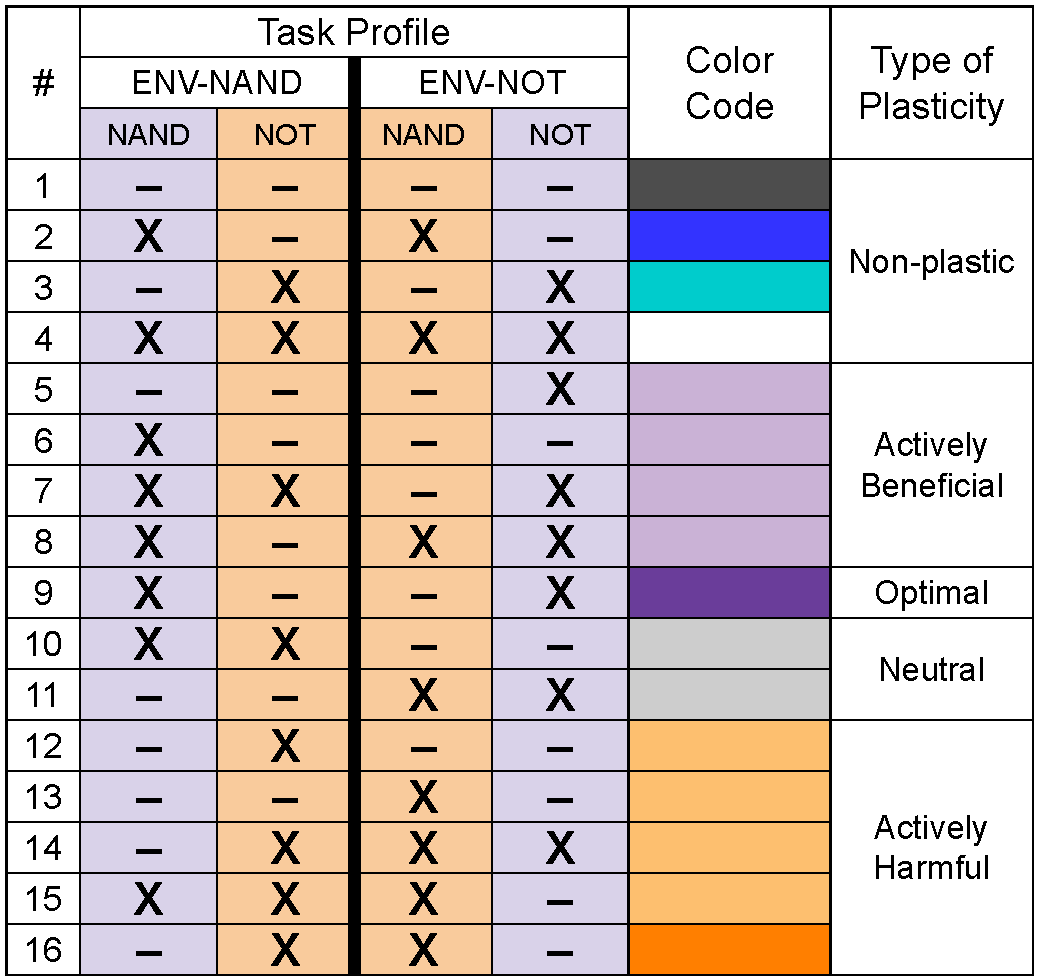
\includegraphics[width=0.75\columnwidth]{chapters/02-evolutionary-origins-of-plasticity/media/task-profiles.pdf}
  \caption{\small 
  Enumeration of all possible complete phenotypes. 
  Each row represents a distinct phenotype. 
  An `X' indicates that the associated task is performed in the specified environment, while a `--' indicates that the task is not performed. 
  For each environment, the column of the rewarded task is highlighted in light purple, and the column of the punished task is highlighted in light orange. 
  An `X' in a reward column or a `--' in the punished column is optimal. 
  Each phenotype has a color code, which is used in our lineage visualization visualizations.  
  Note that the first four rows are non-plastic phenotypes, rows 5--8 exhibit partially beneficial plasticity, and row 9 is optimally beneficial.  
  Rows 10--11 are neutral non-adaptive plasticity, while rows 12--16 are detrimental forms of plasticity.}
  \label{chapter:origins-of-plasticity:fig:task-profiles}
\end{figure*}